\chapter{Языки разработки моделей и~аппаратуры}\label{chapter12}
\dictum[BSV by Example]{When someone comes to you with ``a new language'' it is often time to run the other way\footnotemark}
\footnotetext{Когда кто-то идёт к вам с предложением использовать <<новый язык>>, чаще всего следует развернуться и бежать в противоположном направлении.}

%В данной главе рассматриваются принципы, лежащие в основах специализированных языков, используемых для описания моделей и разработки аппаратуры. Полный обзор всех существующих решений выходит за рамки данного учебника, поэтому будут описаны наиболее популярные в настоящее время языки.
 
Симуляторы и входящие в их состав отдельные модели устройств сами по себе являются программами. Они пишутся на некотором выбранном языке (или нескольких языках) программирования. В законченном симуляторном решении, претендующем на право называться удобным и расширяемым, можно выделить функциональные блоки, различные по своему назначению. Пример структуры некоторого симулятора приведён на рис.~\ref{fig:breakdown}. 
% В зависимости от назначения, развитости проекта состав 
\begin{figure}[h]
    \centering
    % \includegraphics[width=\textwidth]{./breakdown-crop.pdf}
\begin{tikzpicture}[>=latex, font=\small]
    \node[] (gui) {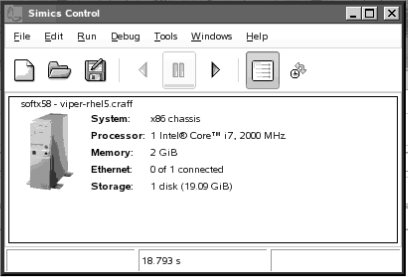
\includegraphics[width=2cm]{./gui.png}};
    \node[above=0.1cm of gui] {Графический интерфейс};
    
    \node[right = 1cm of gui]     (device1) {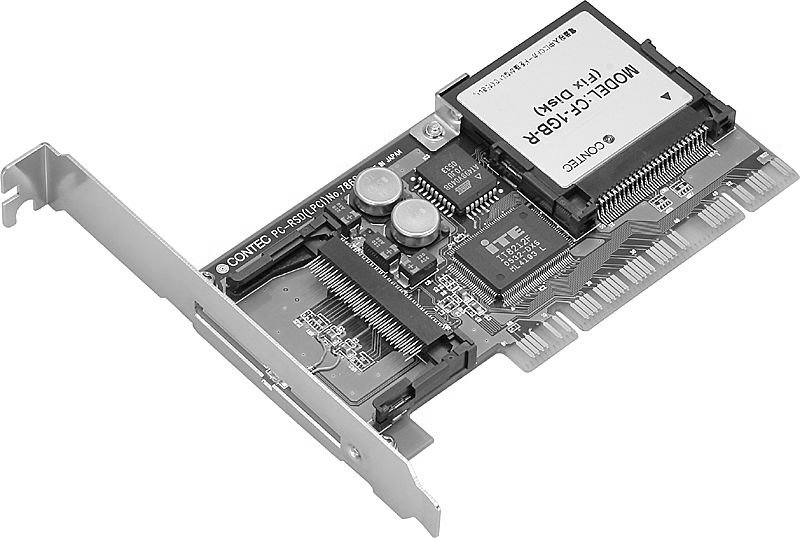
\includegraphics[height=1.5cm]{./device1.png}};
    \node[right = 0.2cm of device1] (device2) {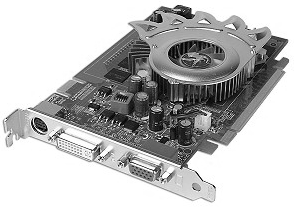
\includegraphics[height=1.5cm]{./device2.png}};
    \node[right = 0.2cm of device2] (device3) {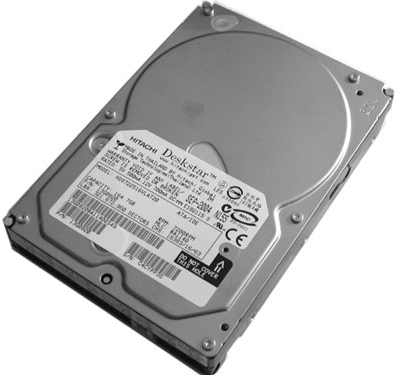
\includegraphics[height=1.5cm]{./device3.png}};
    
    \node[draw, inner sep= 2pt, fit=(device1) (device3)] (frame) {};
    
    \node[below = 2.5cm of gui] (cli) {
\includegraphics[height=1.5cm]{./cli.png}};
    
    \node[draw, circle, below = 0.7cm of device1] (core) {Ядро};
    
    \node[right = 3cm of cli] (python) {
\includegraphics[height=1.5cm]{./python.png}};
    \node[right = 0.2cm of python] (perl) {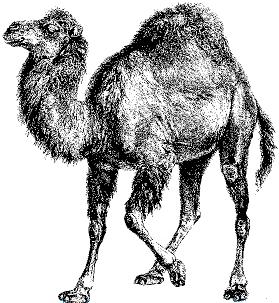
\includegraphics[height=1.5cm]{./perl.png}};
    \node[right = 0.2cm of perl] (lua) {
\includegraphics[height=1.5cm]{./lua.png}};
    
    \node[above=0.1cm of cli] {Командная строка};
    \node[above=0.1cm of perl] {Язык сценариев};
    \node[above=0.1cm of device2] {Модели устройств};
    
    \draw[<->, shorten >=0.8cm] (core) -- (gui);
    \draw[<->, shorten >=0.2cm] (core) -- (frame);
    \draw[<->, shorten >=0.8cm] (core) -- (cli);
    \draw[<->, shorten >=0.8cm] (core) -- (perl);
\end{tikzpicture}
    \caption[Структура и классификация компонент симулятора]{Структура и классификация компонент симулятора. Графический интерфейс и командная строка отвечают за взаимодействие с пользователем. Языки сценариев (скрипты) обеспечивают средства автоматизации и расширения функциональности. Модели устройств используются для конструирования изучаемой системы. Ядро связывает компоненты в единое целое}
    \label{fig:breakdown}
\end{figure}

Каждая из компонент симулятора может быть реализована на своём языке, наиболее адекватном требуемой функциональности. Например, графический интерфейс может быть сделан с помощью библиотек (языков) Qt (С++), AWT (Java), Tk (Tcl) и т.д. Интерпретатор сценариев, скорее всего, будет выполнен на том же динамическом языке, который предполагается использовать для написания скриптов.

Перейдём к основной части любого симулятора --- моделям устройств. Для их создания можно использовать языки общего назначения, такие как Си, Си++. Их универсальность и гибкость позволит написать каждую модель «с нуля». При этом придётся самостоятельно вводить все необходимые абстракции предметной области симуляции, вычленять иерархическую структуру создаваемой системы и сопоставлять её с возможностями языка.

Однако специфика задачи моделирования такова, что является возможным выделение некоторых абстракций в законченные модули, удобные для повторного использования, и интеграции моделей, написанных разными людьми, с помощью набора документированных интерфейсов. При этом возникает возможность переиспользования части работы, уже выполненной кем-то. По этой причине в индустрии программного моделирования можно выделить два подхода.

\paragraph{Создание библиотек для языков общего назначения, реализующих необходимые для  моделирования примитивы.} В этом случае желаемые понятия формулируются в терминах типов данных, функций или объектов, полей и методов для объектно-ориентированных языков. У разработчика, использующего такую систему, остаётся полная свобода выражения, ограниченная лишь синтаксисом применяемого языка.
\paragraph{Использование специализированных языков описания моделей.} Концепции моделирования вносятся в ядро языка, что уменьшает сложность создаваемых кодов и повышает темп разработки. Однако требуется некоторое время и усилия для того, чтобы разработчики освоили новый язык.

Сходная задача возникает перед разработчиками аппаратуры: описывать работу цифровых схем. В этом случае языки общего назначения применимы ещё меньше, так как оперируют не теми базовыми абстракциями; практически всегда используются языки специализированные. Однако при этом преследуется цель, отличная от задач моделирования: требуется получить структуру, из которой возможно генерировать описание физического расположения элементов на кристалле разрабатываемой микросхемы, пригодного для изготовления настоящих экземпляров устройства на фабрике. Генерация симулятора системы по описанию аппаратуры также возможна и широко используется на финальных этапах разработки. Степень детализации подобной симуляции часто превышает необходимую, и модель получается чрезвычайно медленной. Это, в том числе, ограничивает масштаб модели одной или несколькими микросхемами, тогда как часто требуется симулятор, содержащий в себе весь комплекс целиком.

\section{Разработка моделей}

Всякий язык высокого уровня призван сделать процесс разработки программ определённого типа менее сложным, чем это представляется при использовании языков данной машины --- ассемблера или двоичного машинного кода. Достигается такое упрощение введением некоторых понятий, часто применяемых в целевой программе, и переформулированием их в виде, удобном для человека. Например, в спецификации языка Си можно увидеть такие понятия, как переменная, имеющая имя (в машинном коде есть только безымянные ячейки памяти), типы, логически выстраивающие структуру данных, функции, объединяющие в себе действия, часто совершаемые совместно в фиксированном порядке и т.п. 

\subsection{Требования на языки}

Абстракции языков общего назначения применимы для широкого класса программ, которые можно на них писать. Области моделирования аппаратуры и проектирования цифровых схем используют более узкий набор понятий. Именно их требуется представлять в \emph{предметно-ориентированных языках} (\abbr domain specific languages). Перечислим некоторые абстракции, часто встречаемые в аппаратуре, но не в программах общего назначения. 

\paragraph{Сигналы.} Простейший сигнал --- это логический уровень (\abbr level), кодирующий логическую единицу или ноль. В физических системах он может присутствовать на проводнике, соединяющем части схемы. Также сигналом может быть факт изменения (т.н. фронт, \abbr edge) с высокого уровня на низкий или наоборот.

\paragraph{Шины.} За один такт между частями некоторой схемы может требоваться передать не один бит информации, а несколько. При этом набор проводников объединяется в логическую группу из нескольких независимых однобитных сигналов, образующих \emph{шину} (\abbr bus).

\paragraph{Операции над отдельными битами чисел.} Базовая функциональность операций над битами присутствует во многих языках общего назначения, включая Си. Однако описание функций аппаратуры часто требует большего разнообразия доступных функций, как то: операции над диапазонами бит, применение масок, сдвиги, обработка чисел с шириной, не кратной восьми, и т.д.

\paragraph{Транзакции.} Отражают мгновенность акта передачи нескольких сигналов по шине, а также направление сигнала (т.е. наличие отправителя и получателя).

\paragraph{Расширенные значения для уровней сигналов.} Традиционная Булева алгебра подразумевают существование только двух значений для величин --- <<истина>> (единица, высокое напряжение и т.д.) и <<ложь>> (ноль, низкое напряжение и т.д.). При проектировании цифровой аппаратуры в описаниях логики работы узлов могут использоваться дополнительные состояния. Например, следующие два определены в стандарте Verilog.
\begin{enumerate*}
\item Неопределённое, или X. Фактический уровень сигнала не влияет на работу схемы.
\item Высокий импеданс, или Z. Контакт не подключен ни к одному выходу схемы, или же сопротивление между ним и выходом очень велико.
\end{enumerate*}

\paragraph{Абстракции хранения данных.} Среди них следует выделить одиночные и группы регистров разной ширины, каналы (FIFO), банки памяти различной ёмкости.

\paragraph{Карты памяти.} Обращение некоторого устройства по адресу в памяти может быть обработано различными устройствами в зависимости от значения адреса; при этом правило определения обработчика может быть сложным или динамически зависеть от сторонних условий.

%\paragraph{Побочные эффекты} от обращения к регистрам при чтении и записи. 

\paragraph{Виртуальное время.} Часто модель требует для своей работы наличие монотонно изменющегося счётчика времени, не зависящего от течения физического времени. Со всеми операциями моделируемой систему при этом ассоциированы некоторые задержки в терминах этого времени.

\paragraph{Параллельная обработка.} В синхронных цифровых схемах все узлы работают одновременно и независимо при поступлении сигнала с тактового генератора. При этом каждый обрабатывает данные с предыдущего такта и формирует результаты, которые будут доступны на следующем такте. Это --- специфический вид параллелизма, который можно использовать при симуляции для её ускорения.

\subsection{SystemC}

Необходимые для деятельности разработчика моделей абстракции могут быть выражены в терминах универсального языка программирования и затем оформлены в модули и библиотеки. Эти <<кирпичики>> затем могут быть использованы для создания моделей. При этом возможности использованного языка не исчезают --- их можно продолжать использовать, если в этом возникает необходимость.

Именно таким образом организован \textbf{SystemC} --- <<язык>> проектирования и верификации моделей системного уровня, реализованный в виде библиотеки C++, которая включает компоненты дискретного моделирования событий~\cite{systemc2006}. 

SystemC курируется организацией <<Accelera Systems Initiative>>, созданной в 2011 году в результате объединения двух организаций, разрабатывающих стандарты в области автоматизации проектирования электронных систем: Accelera и Open SystemC Initiative. Он был принят ассоциацией IEEE как стандарт IEEE 1666-2005, обновленный в 2011 году как IEEE 1666-2011. Существует «эталонная» реализация данной библиотеки, однако большое количество компаний-разработчиков аппаратуры  выпустили свои реализации и инструменты. Все они основаны на общих спецификациях и поэтому совместимы.

\paragraph{TLM} Первая версия SystemC решала задачи моделирования, подходя к ним со стороны задачи описания аппаратуры. Поэтому в него были включены возможности и аспекты, характерные для языков описания аппаратуры: иерархическое построение и соединение модулей, потактовая точность, использование дельта-циклов для упорядочивания событий, поддержка четырёхзначной логики и т.п.
В дальнейшем акцент языка сдвинулся на более высокие уровни абстракции: представления для передачи сообщений и моделирования полных платформ. Это расширение было осуществлено согласно принципам \textbf{TLM} (\abbr Transaction Level Modeling)~\cite{tlm2003} и вошло во вторую версию стандарта SystemC. 

\subsubsection{Архитектура}
\dictum[Joel Spolsky]{All non-trivial abstractions, to some degree, are leaky\footnotemark}
\footnotetext{Все нетривиальные абстракции в некоторой степени <<протекают>>}

Язык использует возможности нижележащего С++ для объектной декомпозиции разрабатываемых моделей. Возможности определения шаблонных классов используются для описания часто используемых при моделировании абстракций. Например, в SystemC определены такие типы, как \texttt{sc_bv<>} --- вектор бит, и \texttt{sc_lv<>} --- вектор четырёхзначных сигналов.

На рис.~\ref{fig:systemc-arch} отображены типы, инструменты и уровни представления систем, доступные при использовании SystemC. Разработчик модели сам определяет абстракции, которые он будет использовать.

\begin{figure}[htb]
    \centering
    % 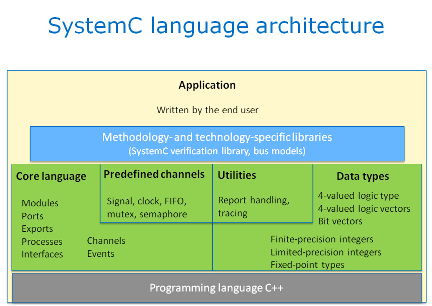
\includegraphics[width=\textwidth]{./tmp/systemc-arch.png}
\begin{tikzpicture}[scale=1.13, >=latex, font=\footnotesize]
    \coordinate (a01) at (-5 ,0.5);
    \coordinate (a02) at ( 5 ,0.5);
    \coordinate (a03) at (-5  ,-1);
    \coordinate (a04) at (-2.5,-1);
    \coordinate (a05) at (   0,-1);
    \coordinate (a06) at ( 2.5,-1);
    \coordinate (a07) at (   5,-1);
    \coordinate (a08) at (   0,-2);
    \coordinate (a09) at (  -5,-3);
    \coordinate (a10) at (   0,-3);
    \coordinate (a11) at (   5,-3);
    \coordinate (a12) at (   5,-3.5);
    
    \coordinate (b01) at (-4.5,-0.5);
    \coordinate (b02) at ( 4.5,  -1);
    
    \coordinate (l01) at ( 0,   0);
    \coordinate (l02) at ( 0,-0.75);
    \coordinate (l03) at (-2.5,-1.5);
    \coordinate (l04) at ( 0,-1.5);
    \coordinate (l05) at (-5, -1);
    \coordinate (l06) at ( 2.5, -1);
    \coordinate (l07) at (   0,-3.25);
    
    \draw (a01) rectangle (a12);
    \draw (b01) rectangle (b02);
    
    \draw (a03) rectangle (a10);
    \draw (a04) rectangle (a08);
    
    \draw (a05) rectangle (a11);
    \draw (a08) rectangle (a06);
    \draw (a09) rectangle (a12);
    
    \node at (l01) {Приложение};
    \node at (l02) {Библиотеки, специфичные для выбранной технологии};
    \node[align=left, text width=3cm, anchor = west] at (l03) {Каналы: signal, clock, FIFO, mutex, semaphore};
    \node[align=left, text width=3cm, anchor = west] at (l04) {Утилиты: \\ трассировка, \\ отчёты};
    
    \node[align=left, text width=3cm, anchor = north west] at (l05) {Язык: модули, порты, экспорты,\\ процессы,\\ интерфейсы, каналы, события};
    \node[align=left, text width=3cm, anchor = north west] at (l06) {Типы данных: \\ 4-значная логика, вектора, целые и действительные\\ числа};
    
    \node at (l07) {Язык С++} ;

\end{tikzpicture}
    \caption[Архитектура приложения на SystemC]{Архитектура приложения на SystemC}
    \label{fig:systemc-arch}
\end{figure}

\subsubsection{Пример}

Пример кода, использующего SystemC\footnote{Приведённые ниже примеры кода на языках SystemC, Verilog  и VHDL взяты из Wikipedia.}.

\begin{lstlisting}
#include "systemc.h"
SC_MODULE(adder) {        // module (class) declaration
  sc_in<int> a, b;        // ports
  sc_out<int> sum;
  void do_add() {         // process
    sum.write(a.read() + b.read()); //or just sum = a + b
  }
  SC_CTOR(adder) {        // constructor
    SC_METHOD(do_add);    // register do_add to kernel
    sensitive << a << b;  // sensitivity list of do_add
  }
};
\end{lstlisting} 

\subsubsection{Сборка модели}

Процесс сборки SystemC-модели из исходных кодов не отличается от аналогичного процесса для программы на С++. Исходные коды компилируются в объектные файлы, которые затем объединяются редактором связей (линкером) вместе с библиотеками SystemC и другими зависимостями в исполняемое приложение (рис.~\ref{fig:systemc-compilation})

\begin{figure}[htb]
    \centering
% 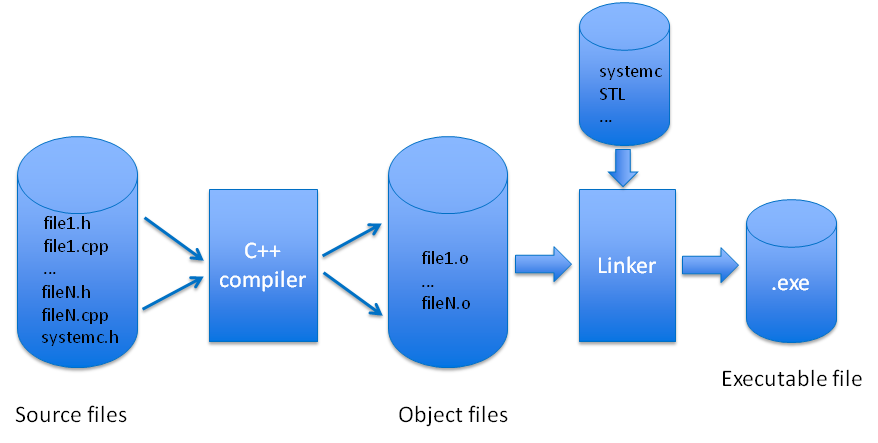
\includegraphics[width=\textwidth]{./tmp/systemc-compilation.png}
\begin{tikzpicture}[scale=1.0, >=latex, font=\small]

\begin{scope}[text width=1.4cm]
    \node[draw, rounded corners] (file1-h) {file1.h};
    \node[draw, rounded corners, below= 0cm of file1-h.south west, anchor=north west] (file1-cpp) {file1.cpp};
    \node[draw, rounded corners, below= 0cm of file1-cpp.south west, anchor=north west] (fileN-h) {fileN.h};
    \node[draw, rounded corners, below= 0cm of fileN-h.south west, anchor=north west] (fileN-cpp) {fileN.cpp};
    \node[draw, rounded corners, below= 0cm of fileN-cpp.south west, anchor=north west] (systemc-h) {systemc.h};
\end{scope}
    
\node[draw, right = 0.5cm of fileN-h, text width=1.8cm, align=center] (compiler) {C++ \\ компилятор};

\begin{scope}[text width=1.cm]
    \node[draw, rounded corners, right= 3.2cm of file1-cpp] (file1-o) {file1.o};
    \node[draw, rounded corners, right= 3.2cm of fileN-cpp] (fileN-o) {fileN.o};
\end{scope}

\node[draw, right = 2.6cm of compiler,] (linker) {Линкер};
\node[draw, rounded corners, above = of linker, align=center] (libs) {SystemC \\ библиотеки};

\node[draw, rounded corners, right = 0.5cm of linker, align=center, fill=black!10] (exe) {Исполняемый\\файл};

\draw[->] (file1-h.east) -- (compiler);
\draw[->] (file1-cpp.east) -- (compiler);
\draw[->] (fileN-h.east) -- (compiler);
\draw[->] (fileN-cpp.east) -- (compiler);
\draw[->] (systemc-h.east) -- (compiler);
    
\draw[->] (compiler) -- (file1-o);
\draw[->] (compiler) -- (fileN-o);

\draw[->] (file1-o) -- (linker);
\draw[->] (fileN-o) -- (linker);

\draw[->] (libs) -- (linker);
\draw[->] (linker) -- (exe);

\end{tikzpicture}
    \caption[Сборка модели SystemC]{Последовательность сборки модели SystemC из исходных кодов}
    \label{fig:systemc-compilation}
\end{figure}

% \subsubsection{Планировщик симулируемого времени SystemC}

% \todo Описать

% Управляет исполнением процессов

% Дискретно событийный

% Невытесняющая многозодачность

% Детерминистичен относительно событий, упорядоченных во времени

% 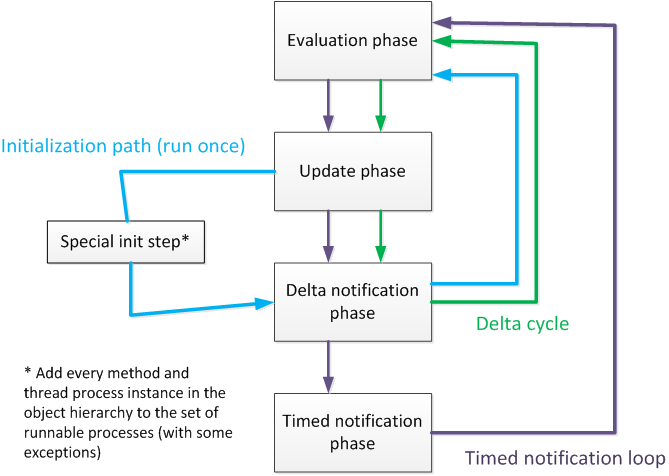
\includegraphics[width=\textwidth]{./tmp/systemc-scheduler.png}

\subsection{Специализированные языки}

Для решения специфических задач существуют предметно-ориентированные языки, предназначенные для разработки аппаратуры. Их использование рационально при условии, что они задействованы как часть большого пакета для моделирования систем.

\paragraph{Пример: DML}

Другим примером языка, специально созданного для описания функциональных моделей устройств, является DML (Device Modeling Language), используемый в симуляторе Simics~\cite{dml-tutorial}, в котором упор сделан на максимально быстрое модельное прототипирование устройств, т.е. создание заготовки устройства, не имеющей полной функциональности, но предоставляющей все внешние интерфейсы реального устройства. Этот подход позволяет реализовывать сложные системы постепенно, притом концентрироваться на самых  важных функциональных аспектах в первую очередь и дописывать недостающие компоненты после. Основной тип устройств, описываемых с помощью DML, --- это неисполняющие устройства, он не используется для создания моделей процессоров.

Синтаксис DML предоставляет программисту конструкции для описания банков регистров, интерфейсов и функционального поведения устройств. Использование DML для написания модели автоматически гарантирует многие декларируемые Simics свойства у получаемых моделей.

\begin{itemize*}
\item Явное представление архитектурного состояния в \textit{атрибутах}.
\item Корректное сохранение и загрузка состояния симуляции из точек сохранения.
\item Безопасная многопоточность (\abbr thread safety).
\item Поддержка правильного порядка байт данных (т.н. Endianness) при взаимодействии моделей между собой.
\item Генерация текста документации из комментариев и строк описания деталей модели.
\end{itemize*}

Существующий компилятор \texttt{DMLC} является т.н. source-to-source компилятором, т.е. результатом его работы являются не машинные инструкции, а промежуточный текст на языке Си, который затем обрабатывается компилятором GCC. Однако при этом двухстадийном процессе сохраняется отладочная информация о строках исходного DML-кода, что позволяет использовать специально модифицированный вариант отладчика GDB, «понимающего» синтаксис DML для работы с исходным, а не с промежуточным кодом при отладке. Дополнительно этот подход позволяет при необходимости с помощью специальных команд языка включать код на Си в программу на DML, при этом такие куски передаются в промежуточный код без изменений.

\textbf{Пример кода на DML} % dammit I don't know why \paragraph does not work.

\begin{lstlisting}
register lcr { 
  parameter soft_reset_value = 0x00; 
  parameter hard_reset_value = 0x00; 
  field wls          [1:0] "Word length select "; 
  field stb          [2] "Number of stop bits (0 = 1, 1 = 2)"; 
  field pen          [3] "Parity enable (0 = disable, 1 = enable)"; 
  field eps          [4] "Even parity select (0=Odd, 1=Even)"; 
  field stick_parity [5] "Stick parity"; 
  field set_break    [6] "Set break"; 
  field dlab         [7] "Divisor latch access bit"; 
  // After a write to this register, check the contents of WLS and  
  // set the character length mask appropriately 
  method after_write (memop) { 
    if      ($wls == 0) $mask = 0x1F; 
    else if ($wls == 1) $mask = 0x3F; 
    else if ($wls == 2) $mask = 0x7F; 
    else                $mask = 0xFF; 
  } 
}   
\end{lstlisting} 


\subsection{Языки описания набора инструкций}

Отдельное внимание следует уделить разработке моделей процессоров и языкам, предназначенным для их создания.

Сложность данной задачи заключается в том, что при разработке совершенно нового устройства его авторам требуется иметь в рабочем состоянии одновременно  несколько инструментов и документов из следующего списка:

\begin{itemize*}
\item функциональный симулятор набора инструкций;
\item точная потактовая модель;
\item дизассемблер машинного кода;
\item компилятор с языка высокого уровня в машинный код;
\item документация к аппаратуре;
\item иногда необходимо также уметь генерировать синтезируемое описание новой архитектуры.
\end{itemize*}

Если каждая компонента разрабатывается отдельно, то при изменении спецификации процессора (что происходит часто на ранних этапах исследования) приходится вносить изменения во всех программах и документах, что чревато ошибками и десинхронизацией инструментов, каждый из которых фактически имеет собственный «взгляд» на одно и то же устройство.  

Существует несколько проектов языков, призванных решить всю описанную задачу. В качестве примера см. LISA~\cite{wahlen2004c,zivojnovic1996,schliebusch2002}, ISDL~\cite{Hadjiyiannis97isdl:an,isdl1997} и~\cite{hoffmann2001}. Решение состоит в автоматической генерации необходимых инструментов из одного описания (рис.~\ref{fig:lisa}). 

\begin{figure}[htb]
    \centering
%     \includegraphics[width=0.5\textwidth]{./lisa-crop.pdf}
\begin{tikzpicture}[>=latex, font=\small]
\def\gear{
    \begin{tikzpicture}
    \draw[scale=1]
    \foreach \i in {1,2,...,10} {% draw the gear
        [rotate=(\i-1)*36]  (0:0.5)  arc (0:12:0.5) -- (18:0.7)  arc (18:30:0.7) --  (36:0.5)
    };
    \end{tikzpicture}
}
    \node[draw, tape] (src) {Исходное описание}
    [level distance=2cm, sibling distance=2.5cm, edge from parent/.style={draw, ->}]
    child {node[] {\gear}
        child {node {Дизассемблер}}
    }
    child {node[] {\gear}
        child {node {Симулятор}}
    }
    child {node[] {\gear}
        child {node {Документация}}
    };
\end{tikzpicture}
    \caption{Генерация инструментов разработки из общего описания архитектуры}
    \label{fig:lisa}
\end{figure}


Одним из недостатков этого подхода является зачастую субоптимальная скорость или качество работы получаемых инструментов; например, компилятор может генерировать не самый быстрый или компактный код, функциональная модель работает медленнее, чем могла бы будучи написанной человеком, синтезируемое описание занимает излишне много места на кристалле и т.д. Тем не менее скорость создания, модификации и степень согласованности всех инструментов часто перевешивают эти огрехи на ранних этапах, а затем, после фиксации спецификаций, все инструменты могут быть переписаны «вручную», с необходимыми оптимизациями.

Другой аспект, возникающий при создании моделей процессоров --- желание иметь её с более чем одним механизмом симуляции, например, создать интерпретатор и двоичный транслятор и затем иметь возможность переключаться между ними. И снова для того, чтобы избежать рассинхронизации суб-моделей при правках спецификаций, чаще всего избирается подход,  при котором они генерируются из одного описания семантики инструкций~\cite{simgen}.

Для построения двоичных трансляторов также может использоваться преобразование описаний семантики гостевых инструкций в заготовки машинного кода, при этом исходное описание является неким метаассемблером, преобразуемым в настоящий ассемблер хозяйской архитектуры (рис.~\ref{fig:capsules}). Такой подход позволяет разработчику иметь наибольший контроль над создаваемым двоичным транслятором~\cite{MyConfMIPT52}. Существенным недостатком является полная непереносимость модели на другую хозяйскую архитектуру, т.к. при этом приходится переписывать весь код эмуляции инструкций.

\begin{figure}[htb]
    \centering
%     \includegraphics[width=0.75\textwidth]{./capsules-crop.pdf}
\begin{tikzpicture}[>=latex, font=\small]
\def\gear{
    \begin{tikzpicture}
    \draw[scale=1]
    \foreach \i in {1,2,...,10} {% draw the gear
        [rotate=(\i-1)*36]  (0:0.5)  arc (0:12:0.5) -- (18:0.7)  arc (18:30:0.7) --  (36:0.5)
    };
    \end{tikzpicture}
}
\node[draw, tape, text width=9cm, align=left, font=\footnotesize\ttfamily] (src){
NJU(U32 @Curr_IP, U32 @op_size, X128 @ireg_dst)\\
\{\\
@UPDATE_Curr_IP(@Curr_IP)\\
\ \ \ \ movl  \$@op_size,  @glst_arg0_w0(\%ebp)\\
\ \ \ \ cmpss \$0xffff, (\%esi), @ireg_dst\\
\}\\
};

\node[above=0.15cm of src] {Исходное описание};

\node[below=0.5cm of src] (gear) {\gear};

\node[minimum height=1.8cm, inner sep=2pt, below=0.5cm of gear, xshift=-3cm, draw, tape, text width=4cm, align=left, font=\scriptsize\ttfamily] (asm){
movl  \$0xdeadc0de,  12(\%ebp) \\
cmpss \$0xffff, (\%esi), \%ebx \\
};

\node[below=0.15cm of asm] {Ассемблер};

\node[minimum height=1.8cm, inner sep=2pt, below=0.5cm of gear, xshift=3cm, draw, tape, text width=4.5cm, align=left, font=\scriptsize\ttfamily] (emitter){
\#define NJU\textbackslash\\
(Curr_IP, op_size, ireg_dst)\textbackslash \\
...
};
\node[below=0.15cm of emitter] {Эмиттер};

\draw[->] (src) -- (gear);
\draw[->] (gear) -- (asm);
\draw[->] (gear) -- (emitter);
\end{tikzpicture}
    \caption[Создание двоичного транслятора из метаассемблера]{Создание двоичного транслятора из метаассемблера. Исходное описание содержит в себе аргументы создаваемой функции и ассемблерные инструкции хозяйской архитектуры. После процесса обработки мы имеем два блока исходного кода --- ассемблерный код, используемый при симуляции, а также код на Си (эмиттер), передающий первому аргументы на этапе трансляции}
    \label{fig:capsules}
\end{figure}


% \subsection{Bluespec}

% \todo Описать.

% Arvind had developed the Bluespec language, a high-level functional hardware description programming language which was essentially Haskell extended to handle chip design and electronic design automation in general. Bluespec is partially evaluated (to convert the Haskell parts) and compiled to the term rewriting system. The justification behind writing chip designs in Bluespec is that it leads to shorter, more abstract, and verifiable (provably correct) source code, as well as type-checked numeric code. Bluespec, Inc. claims greater than 50\% improvements compared to conventional methods of design[citation needed]. It also comes with a SystemVerilog frontend.

% Bluespec is the only ESL synthesis solution for control logic, complex datapaths and algorithms[citation needed]. For SystemC users, Bluespec has delivered high-level ESL Synthesis abstractions to SystemC. Bluespec integrates seamlessly into Cadence, Synopsys, Mentor and Magma flows, including verification, debug and synthesis, without requiring new methodologies or tools.


\section{Языки разработки аппаратуры}

В заключение кратко познакомимся с двумя самыми популярными языками описания аппаратуры (\abbr Hardware Definition Language, HDL), используемыми в настоящее время --- Verilog и VHDL.

\subsection{Verilog}
 
Verilog был создан Филом Мурби и Прахбу Гоелом в  1984 году в фирме Auto\-mated In\-te\-gra\-ted De\-sign Sys\-tems. Он был принят как стандарт IEEE 1364-1995. Позже дополнения к языку Verilog-95 были приняты как IEEE 1364-2001 (или Veri\-log-2001). Следующий вариант, Verilog 2005 (стандарт IEEE 1364-2005), добавил небольшие исправления, уточнения спецификаций и несколько новых синтаксических конструкций.

Разработчики Verilog сделали его синтаксис очень похожим на синтаксис языка C, что упрощает освоение. Язык имеет препроцессор, очень похожий на препроцессор языка C, и основные управляющие конструкции \texttt{if}, \texttt{while} также подобны одноимённым конструкциям языка C. 

Существует подмножество инструкций языка Verilog, называемое синтезируемым. Модули, которые написаны на этом подмножестве, называют \textit{RTL} (\abbr register transfer level --- уровень регистровых передач). Они могут быть физически реализованы с использованием САПР-синтеза. Данные САПР по определённым алгоритмам преобразуют абстрактный исходный код на Verilog в \emph{netlist} --- логически эквивалентное описание, состоящее из элементарных логических примитивов (например, AND, OR, NOT, триггеры), которые доступны в выбранной технологии производства СБИС или программирования БМК и ПЛИС. Дальнейшая обработка netlist в конечном итоге порождает фотошаблоны для литографии или прошивку для FPGA.

Что отличает этот язык от обычных языков общего назначения? Во-первых, разделение всех команд на \textit{синтезируемые}, т.е. непосредственно представляемые в аппаратуре, и на \textit{несинтезируемые}, используемые только для отладки и симуляции.

Оператор \texttt{<=} в Verilog является ещё одной особенностью языка описания аппаратных средств, отличающей его от процедурных языков общего назначения. Сама операция известна как \textit{неблокирующее присваивание}. Применение оператора не имеет внешне видимого эффекта до наступления следующего такта. Это означает, что порядок таких присваиваний в коде не может влиять на суммарный эффект функции, т.к. все они произойдут одновременно и произведут тот же результат: значения \texttt{flop1} и \texttt{flop2} будут обмениваться значениями на каждом такте.

Другой оператор присваивания, <<\texttt{=}>>, является блокирующим. Когда он используется, переменная с его левой стороны обновляется немедленно. В приведённом выше примере, если бы использовался <<\texttt{=}>> вместо <<\texttt{<=}>>, \texttt{flop1} и \texttt{flop2} не обменялись бы значениями. Вместо того, как и в традиционном процедурном программировании, компилятор воспринял бы это как указание сделать их содержимое одинаковым.

\textbf{Пример кода на Verilog: триггер} % dammit I don't know why \paragraph does not work.

\begin{lstlisting}
module toplevel(clock,reset);
 input clock;
 input reset;
 reg flop1;
 reg flop2;
 always @ (posedge reset or posedge clock)
 if (reset)
   begin
     flop1 <= 0;
     flop2 <= 1;
   end
 else
   begin
     flop1 <= flop2;
     flop2 <= flop1;
   end
endmodule         
\end{lstlisting}

\paragraph{SystemVerilog} \cite{systemverilog-ru} --- язык описания и верификации аппаратуры, являющийся расширением языка Verilog, вобравший в себя некоторые черты других языков описания аппаратуры: Superlog и OpenVera. Язык был стандартизирован как IEEE 1800—2005, а позднее он был объединён с Verilog в единый язык (стандарт IEEE 1800—2009). Были добавлены новые типы данных, представлена концепция интерфейсов, используемых для группировки портов. Главным расширением языка по сравнению с Verilog является введение средств для проведения верификации моделей, основанных на объектно-ориентированной парадигме. При этом новые конструкции не входят в синтезируемое подмножество языка.

\subsection{VHDL}

VHDL был разработан в 1983 г. по заказу Министерства обороны США с целью формального описания логических схем для всех этапов разработки электронных систем, начиная с модулей микросхем и заканчивая крупными вычислительными системами.

Первоначально язык предназначался для моделирования, но позднее из него было выделено синтезируемое подмножество. Средствами языка VHDL возможно проектирование на различных уровнях абстракции (поведенческом или алгоритмическом, регистровых передач, структурном) в соответствии с техническим заданием и предпочтениями разработчика. Представляется возможным выделить следующие три составные части языка: алгоритмическую, основанную на языках Ada и Pascal и придающую языку VHDL свойства процедурных языков, и проблемно ориентированную, обращающую VHDL в язык описания аппаратуры, а также объектно-ориентированную, интенсивно развиваемую в последнее время.

\textbf{Пример кода на VHDL} % dammit I don't know why \paragraph does not work.

\begin{lstlisting}
-- latch template 1:
Q <= D when Enable = '1' else Q;
-- latch template 2:
process(D,Enable)
begin
  if Enable = '1' then
    Q <= D;
  end if;
end process;
\end{lstlisting} 

\iftoggle{hasquiz}{
    \section{\Questions к главе \ref{chapter12}} %\label{chapter12-questions}

\subsection*{Вариант 1}

\begin{questions}

\question[3] Какое утверждение наилучшим образом характеризует термин SystemC?
\begin{choices}
    \choice Компилятор языка Си с дополнениями для моделирования систем.
    \choice Язык программирования, похожий на Си.
    \choice Язык программирования, похожий на С++.
    \correctchoice Набор библиотек для С++.
\end{choices}

\question[3] Язык DML используется для разработки
\begin{choices}
    \correctchoice функциональных моделей,
    \choice потактовых моделей,
    \choice гибридных моделей.
\end{choices}

\question[3] Текущая реавлизация комилятора DMLC является
\begin{choices}
    \choice компилятором типа source-to-source с промежуточным языком С++,
    \choice компилятором, преобразующим исходный текст в байткод Java,
    \correctchoice компилятором типа source-to-source с промежуточным языком Си,
    \choice классическим компилятором,
    \choice частичным интерпретатором.
\end{choices}

\question[3] Закончите фразу: Языки разработки аппаратуры
\begin{choices}
\choice не используются для начального моделирования устройств, так как могут быть преобразованы только в netlist,
\correctchoice не используются для начального моделирования устройств, так как получаемые модели очень медленны,
\choice не используются для начального моделирования устройств, так как могут содержать в себе синтезируюмую часть,
\choice используются для начального моделирования устройств.
\end{choices}

\end{questions}

\subsection*{Вариант 2}

\begin{questions}

\question[3] Какое утверждение наилучшим образом характеризует термин TLM?
\begin{choices}
    \choice Язык программирования, похожий на Си.
    \choice Язык программирования, похожий на С++.
    \choice Среда исполнения моделей DES.
    \correctchoice Расширение стандарта SystemC.
\end{choices}

\question[3] Язык DML используется для разработки
\begin{choices}
    \correctchoice неисполняющих моделей,
    \choice исполняющих моделей,
    \choice как исполняющих, так и неисполняющих моделей.
\end{choices}

\question[3] Какой способ наиболее удобен и надёжен для поддержания набора инструментов моделирования в синхронизированном состоянии при постоянном изменении входной спецификации процессора?
\begin{choices}
    \correctchoice Генерация всех инструментов из единого описания.
    \choice Тщательное сравнение всех инструментов после каждого изменения одного из них.
    \choice Создание одного инструмента, поддерживающего максимальное количество функций.
\end{choices}

\question[3] Закончите фразу: Синтезируемое подмножество языков разработки аппаратуры
\begin{choices}
\choice не может быть использовано для создания netlist и RTL-описаний,
\choice используется только для отладки моделей,
\correctchoice  используется для создания netlist и RTL-описаний.
\end{choices}

\end{questions}

% К каждой лекции должно быть от 8 до 12 задач, у каждой задачи должно быть 3-5 вариантов формулировок примерно одинаковой сложности. Допускается объединение нескольких последовательных лекций в одну тему и подготовка тестов к темам.
% Задачи должны полностью соответствовать материалам лекций, то есть лекциях должно быть достаточно информации для ответа на все вопросы.
% Формулировка каждого варианта задачи должна содержать всю необходимую информацию и не должна ссылаться на тексты внутри лекции, картинки или другие задачи или варианты задачи.
% Правильные ответы выделяются знаком «+» перед их формулировкой. Правильных ответов может быть несколько. Для тестов с несколькими ответами как минимум один ответ должен быть правильным и как минимум один ответ должен быть неправильным. 
% 
% Структура теста к лекции
% 
% \subsection*{Задача 1}
% 
% \paragraph{Вариант 1} 
% 
%     Чему равно 2+2?
%         Ответ 1. 3
%         + Ответ 2. 4
%         …
%         Ответ N. 5
% \paragraph{Вариант 2}
%     Чему равно 2*2?
%         + Ответ 1. 4
%         + Ответ 2. 2+2
%         …
%         Ответ N. 5
% \paragraph{Вариант 3}
% 
%     Чему равно 2-2?
%         Ответ 1. 0
% 
% 
%         
% \section{Просто подборка вопросов}
% 
}{}

\iftoggle{webpaper}{
    \printbibliography[title={Литература}]
}{}


